%----------------------------------------------------------------------
%                        PROJECT DEFINITION
%----------------------------------------------------------------------
\renewcommand{\projnr}{C1}
\renewcommand{\projtitleshort}{Planetesimal precursors in turbulent disks}
\renewcommand{\projauth}{Klahr
, Kley}
%
\setcounter{section}{0}
\noindent{\normalfont\sffamily\Large\bfseries Project \projnr: \projtitleshort}
%
\section{Full title:}
\hspace{1\baselineskip}\\
\centerline{\large ``Planetesimal precursors in turbulent protoplanetary disks''}
%\centerline{\large ''}
%
\section{General information}\mbox{}
\subsection{Principle investigators:}
\hspace{-\baselineskip}\\\noindent
%
{\bfseries\itshape Klahr}, Hubertus, Dr.\\
Research Associate, non-tenure\\
Date-of-birth: 21.07.1966, Nationality: German\\
DFG Code number of latest application (KL 1469/2-1) \\
Max-Planck-Institut f\"ur Astronomie\\
K\"onigstuhl 17\\
69117 Heidelberg\\
Tel: 06221 528 255\\
Fax: 06221 528 246\\
Email: klahr@mpia.de\\
Private address: Jahnstr. 42, 67245 Lambsheim, Tel.: (06233) 50092\\
%
\vspace{1em}\\\noindent
{\bfseries\itshape Kley}, Wilhelm, Prof.~Dr.\\
Professor, tenure\\
Date-of-birth: 19. February, 1958, Nationality: German\\
DFG Code number of latest application (KL 650/7-1)\\
Institut f\"ur Astronomie \& Astrophysik\\
Abt.\ Computational Physics\\
Universit\"at T\"ubingen\\
Auf der Morgenstelle 10\\
72076 T\"ubingen\\
Tel: (07071) 29-74007\\
Fax:  (07071) 29-5094\\
Email: wilhelm.kley@uni-tuebingen.de\\
Private address: Herrenbergerstr. 73, 72070 T\"ubingen, Tel.: (07071) 640085
%

\subsection{Co-investigators within this Forschergruppe:}
\begin{coilist}
\item A.~Johansen (MPIA Heidelberg)
\item N.~Dziourkevitch (MPIA Heidelberg)
\item R.~Speith (CPT, Uni T\"ubingen)
\item D.~Marik (CPT, Uni T\"ubingen)
\end{coilist}


\section{Summary (Zusammenfassung)}
\subsubsection{Summary:} 
In this project we will use direct numerical simulations of turbulence to
study the effect on planetesimal precursors ($\approx$ 1cm - 10m). The goal
is twofold: In one part we will measure turbulent relative velocities in
high resolution local simulations, and in the other part we will determine
the global distribution of solids in the ``weather-pattern'' of turbulent
protoplanetary disks.  Thus, we can determine the key parameters for the
influence of turbulence on planetesimal formation from direct numerical
simulations.  The distribution of planetesimal precursors in the
protoplanetary disk will be derived through global 3D-MHD simulations. We
will also determine the degree to which the precursors can be concentrated
locally in protoplanetary disks in particular in flow features such as
spiral arms, high pressure regions or vortex structures.  In addition we
will derive collision speeds and probabilities as generated by the
turbulence as a function of the particle size of the collision partners and
of the location in the disk. The obtained data are an essential input for
projects B1, B2, B3 and C2, and will also be used for project D2.
%
\subsubsection{Zusammenfassung:} 
%
In diesem Projekt messen wir die Sto{\ss}raten und Geschwindigkeiten
zwi\-sch\-en felsgro{\ss}em Gesteinsmaterial im jungen solaren Nebel.  Diese
Sand bis Felsbrocken gro{\ss}en Objekte werden als das Baumaterial unserer
Planeten angesehen. In einem mittleren Gr\"o{\ss}enregime von 1 Zentimeter
bis 10 Metern Durchmesser ist turbulente Verwirbelung die Haupt\-quel\-le
f\"ur Relativgeschwindigkeiten zwischen Objekten gleicher Gr\"o{\ss}e.  Die
Turbulenz im solaren Nebel (allgemein: Protoplanetare Akkretionscheibe) wird
durch eine Magneto-Rotations-Instabilit\"at (MRI) angetrieben.  Innerhalb
des Projekts sollen die Eigenschaften solcher turbulenten Scheiben
untersucht werden und gleichzeitig die Sto{\ss}raten und Geschwindigkeiten
der eingebetteten Teilchen in Abh\"angigkeit von der Gr\"o{\ss}e der
Sto{\ss}partner und der Position in der Scheibe gemessen werden.  Diese
Messwerte k\"onnen dann direkt f\"ur die theoretischen und experimentellen
Untersuchungen von Einzelst\"o{\ss}en (siehe Projekte B1-B3) verwendet
werden und ist essentiell f\"ur Projekt C2. Sie werden auch im Project
D2 verwendet.
%
\section{State of the art (Stand der Forschung)}
%
Planets are accumulated from  micrometer-sized dust grains that are
embedded in the gas in protoplanetary disks (see Dominik et al.\ 2006 for a
recent review).  The observed infrared radiation from protoplanetary disks
comes primarily from micron-sized grains, although observations at longer
wavelengths show that some disks have large populations of grains with sizes
up to mm and cm (Rodmann et al.\ 2006). Turbulent motions in the gas play a
major role in the dynamics of chemical species and solids, at least as long
as the solids are smaller than a few decameters. Thus, an understanding of
how dust grains and chemical species move under the influence of turbulence
is vital for our understanding of the physical processes that take place in
such disks, and for the observational consequences (Ilgner 2004, Ilgner and
Nelson 2006a,b, Turner et al.\ 2006, Dullemond et al.\ 2006).

A protoplanetary disk is not turbulent a priori (see Klahr et al.~2006 for a
recent review).  Only in the presence of magnetic fields and a sufficient
ionization of the gas, an instability can develop, the magneto-rotational
instability (MRI), see Balbus \& Hawley (1991), which will lead to a state
of saturated turbulence. This turbulence is following a Kolmogorov scaling
and represents nonlinear interactions of waves in a broad spectrum.  At the
same time the turbulence develops certain short lived flow features like
vortex tubes and local pressure fluctuations. But also Coriolis forces are
important because an accretion disk is a rotating system. Thus, large enough
flow features will be in a geostrophic balance, i.e.\ magnetic and thermal
pressure are balanced by the Coriolis forces. This situation is very similar
to the weather pattern on earth.  Such geostrophic large scale features can
be very long lived (Klahr \& Bodenheimer 2003; Fromang \& Nelson 2005)
despite the action of turbulent velocity fluctuations on all smaller scales
down to the dissipation range.

Turbulence plays an important role as a driver of coagulation by causing
relative velocities between grains, in particular for particles beyond 1 mm
in size (V\"olk 1980; Mizuno 1988). The actual values of the turbulent
relative velocities used in simulations of coagulation (see Dominik et al.\
2006 for an overview) are not based on observations or numerical
simulations, but on analytical estimates similar to those of Markiewicz et
al.\ (1991). Our proposed approach to derive the quantities important for
the coagulation process from direct numerical simulations has not been
undertaken yet.
%
\subsubsection{Local Disk Simulations:}
%
In the limit of small grains (whose friction time is much shorter than an
orbital period of the disk at a given radius) the turbulence acts on the
dust purely as diffusion. The turbulent diffusion coefficient for the motion
of the grains is often assumed to be equal to the turbulent viscosity of the
gas flow (Tennekes \& Lumley 1972). Defining the {\it Schmidt number} as
the ratio between turbulent viscosity and turbulent diffusion, this
equality leads to a Schmidt number of unity.  Boosted by today's increased
computational power, and by an increased scientific interest in planet
formation and protoplanetary disks, several investigations have measured the
turbulent diffusion coefficient directly from numerical simulations of
magneto-rotational turbulence (Balbus \& Hawley 1991), the only source of
turbulence that is currently known to be consistently able to drive angular
momentum transport in gravitationally stable protoplanetary disks. The
simulations by Johansen and Klahr (2005) yield a Schmidt number that is
around unity for radial diffusion, whereas Carballido et al.\ (2005) find a
value as high as $10$.  The vertical Schmidt number, as measured both by
Johansen \& Klahr (2005), Turner et al.\ (2006) and by Fromang \&
Papaloizou (2006, gives more consistently a number between 1 and 3. Here, it
is worth to note that Turner et al.\ (2006) consider stratified disks, and
Fromang \& Papaloizou (2006) even include the effect of a dead zone without
turbulence around the mid-plane.  Recently, Johansen, Klahr \& Mee (2006)
show that the Schmidt number depends on the strength of the turbulence and
thus on the initial parameters of the disk, especially the strength of an
imposed vertical magnetic field.
%
\subsubsection{Global Disk Simulations}
%
Due to resolution and computational requirements there exist only a limited
number of global full three-dimensional magneto-hydrodynamic (3D-MHD) accretion
disk calculations.  Most of the simulations have been performed neglecting
the vertical stratification of the disk, and have used a cylindrical
potential where gravity depends only on the distance from the axis of
rotation ($z$-axis).  This setup allows the use of periodic boundary
conditions in the vertical direction and reduces the number of required
gridcells significantly.  Armitage (1998) followed the evolution of such a
global disk with a vertical seed field and obtained $\alpha$-values of the
order $10^{-1}$.  In early global simulations, Hawley (2000) has followed the
evolution of disks in a cylindrical setup and of extended equilibrium tori
with full gravity.  Simulations including diffusivity have been performed by
Arlt \& R\"udiger (2001) who use the full gravity, however in a cylindrical
coordinate system.  Due to the flaring of the disk, only a limited radial
range could be used, and the models cover only very few orbital periods
($\approx 10$).  The interaction with a surrounding atmosphere and the
generation of magnetically driven winds has been studied in 3D global
simulations by Steinacker \& Henning (2001).  Here, the disk has been
threaded by a vertical magnetic field.

In long term simulations of protoplanetary accretion disks the saturation of
the magnetic turbulence has been analyzed, using a cylindrical disk setup
without vertical gravity, by Papaloizou \& Nelson (2003).  They enclosed the
unstable region radially by an inner and outer stable layer where stability
has been achieved by using a constant azimuthal angular velocity (rigid
rotation) in these layers. This clever ``sandwich'' construction shuts off
the source of turbulence (driven by the MRI) in the inner and outer layers
and allows turbulence only in an ``active'' central region.  Using a zero
net flux condition on the magnetic field, the unstable middle region settles
after a few hundred orbital periods into a quasi-stationary state with an
effective $\alpha_{\rm eff} \approx 5 \times 10^{-3}$, which is in agreement
with standard estimates of the viscosity in protoplanetary disks.  In
follow-up simulations the evolution of massive planets embedded in such
turbulent disks have been studied (Nelson \& Papaloizou 2003), as well as
the migration of up to meter sized boulders (Fromang \& Nelson 2005). Their
simulations define presently the state of the art for ``almost'' global MHD
simulations. However, neglecting the vertical stratification of the disk
strongly limits the reliability of their results.
%
\subsubsection{Status summary}
%
The local surface density of solid material is a key parameter for
planetesimal formation. Only high enough ``dust'' surface densities will
lead to a sufficiently rapid growth of micron sized dust grains to kilometer
sized planetesimals. The same high local surface density of planetesimals is
then required to form the cores of the gas giants before the disk is
dissolved.

One possibility to accelerate the formation of planetesimals is to
concentrate the dust locally. Magneto-hydrodynamical turbulent eddies, self
gravity, spiral waves and wakes induced by existing planets will influence
the distribution of solid material and tend to create localized regions of
enhanced dust density (see Dominik et al.\ 2006).

To date there exists no comprehensive picture of how efficient these
different concentration mechanisms operate in protoplanetary disks.
Non-ideal effects (such as ionization degree, radiative cooling and
irradiative heating) and the back-reaction of the ``dust'' on the turbulence
play an important role. Not even vertical stratification has been
implemented yet in the global MHD simulations.

For the smallest dust grains the relative velocities needed for coagulation
are acquired purely by Brownian motion. For larger particles, sources of
relative velocities include differences in the settling speed and the radial
drift. But in particular for equal sized objects in the meter range still
coupled to the gas motion, turbulence induced relative velocities are the
only way that leads to collisions.

Even for very simple equations of state (isothermal configurations) there
are only very few existing simulations, most of them with no or only
approximate vertical gravity.  Here, we will focus on constructing realistic
models of radially and vertically stratified disks locally and globally, and
follow explicitly the evolution of embedded dust particles.
%
\section{Preliminary work (Eigene Vorarbeiten)}
%
In the area of local and global accretion disk simulations both research
groups at the Max-Planck Institute in Heidelberg around Hubert Klahr as well
as in the ``Computational Physics'' group in T\"ubingen (around Wilhelm
Kley) have long standing experience and excellent expertise in
multi-dimensional accretion disk simulations.
%
\subsection{Local Disk Simulations}
%
Currently, we study the diffusion properties of magneto-hydrodynamical
turbulence in {\it local} simulations of protoplanetary disks with a
restricted spatial extent (Johansen \& Klahr 2005; Johansen, Klahr \& Mee
2006).
\begin{figure}
\centering{
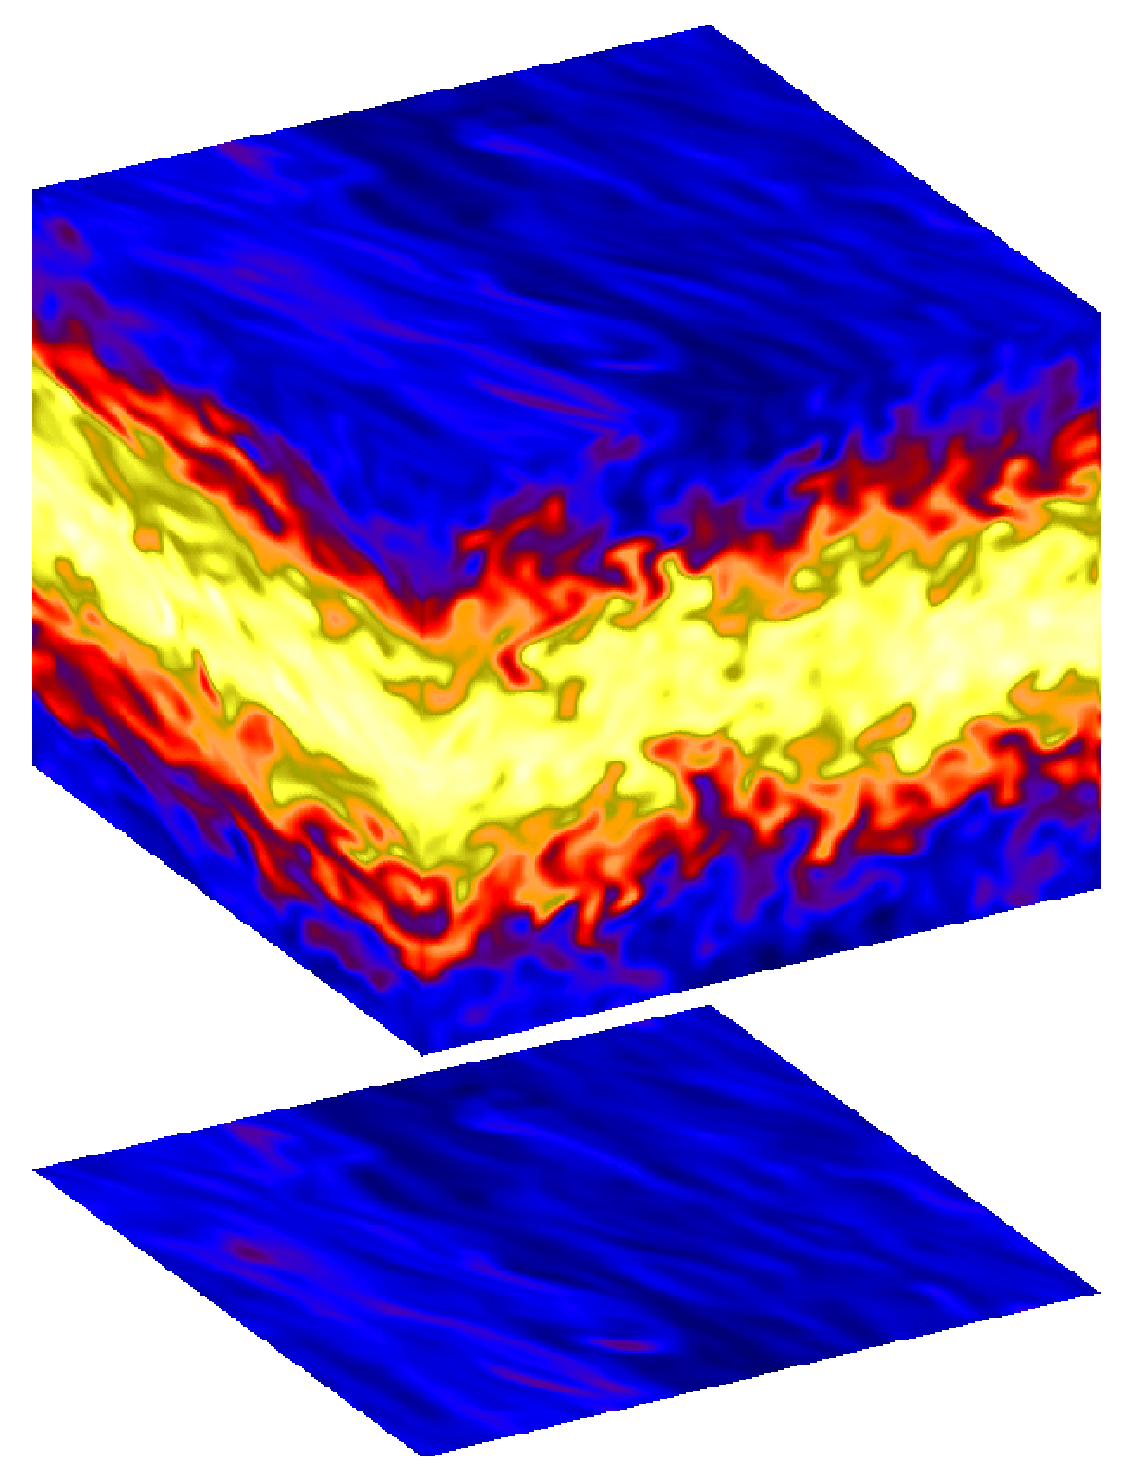
\includegraphics[scale=0.6]{c1fig1.eps}}
\caption{Particle distribution in a turbulent accretion disk. Yellow indicates
a high density around the midplane of the disk, while blue indicates the
depleted upper regions of the disk.  Here we study the equilibrium between
sedimentation and turbulent diffusion.}
\label{fig:c1_1}
\end{figure}
We measure the turbulent diffusion coefficient of dust grains embedded in
magneto-rotational turbulence in a protoplanetary disk directly from
numerical simulations and compare it to the turbulent viscosity of the
flow. The simulations are performed in a local coordinate frame comoving
with the gas which is in Keplerian rotation. Using a two-fluid approach,
small dust grains of various sizes (with friction times up to $\varOmega_0
\tau_{\rm f}=0.02$) are allowed to move under the influence of friction with
the turbulent gas. $\tau_{\rm f}$ is here the stopping time of particles due
to gas drag measured in units of the inverse Keplerian frequency
$\varOmega_0^{-1}$.  A value of $\varOmega_0 \tau_{\rm f}=0.02$ roughly
corresponds to centimeter sized particles at 5 AU in a typical solar nebula.

The turbulent diffusion coefficient of the dust grains is obtained by
applying an external sinusoidal force field acting in the vertical
direction, on the dust component only. This concentrates the dust around the
mid-plane of the disk, and an equilibrium distribution of the dust density
is achieved when the vertical settling is counteracted by the turbulent
diffusion away from the mid-plane. Comparing with analytical expressions for
the equilibrium concentration we deduce the vertical turbulent diffusion
coefficient. It is found to be lower than
the turbulent viscosity and to have an associated vertical diffusion Prandtl
number of about 1.5. A similar radial force field also allows us to measure
the radial turbulent diffusion coefficient. We find a radial diffusion
Prandtl number of about 0.85, and also find that the radial turbulent
diffusion coefficient is abound 70\% larger than the vertical. As most
angular momentum transport happens through magnetic Maxwell stresses, both
the vertical and the radial diffusion coefficients are found to be
significantly larger than suggested by the angular momentum transport due to
Reynolds stresses alone. We also find evidence for trapping of dust grains
of intermediate friction time in turbulent eddies.

We are also interested in the behavior of larger particles (with friction
times around $\varOmega_0 \tau_{\rm f}=1$), and how they are responding to
the turbulence (Johansen, Klahr and Henning 2006).  The value of
$\varOmega_0 \tau_{\rm f} = 1$ corresponds here to meter sized boulders at 5
AU in a typical solar nebula.

In this latter paper we explore the effect magneto-rotational turbulence has
on the dynamics and concentrations of boulders in local box simulations of a
sub-Keplerian protoplanetary disk.  The solids are treated as particles each
with an independent space coordinate and velocity. We find that the
turbulence has two effects on the solids: 1) Meter and decameter bodies are
strongly concentrated, locally up to a factor 100 above the average dust
density, whereas decimeter bodies only experience a moderate density
increase. The concentrations are located in large scale radial gas density
enhancements that arise from a combination of turbulence and shear.  2) For
meter-sized boulders, the concentrations cause the average radial drift
speed to be reduced by $40\%$.  We find that the densest clumps of solids
are gravitationally unstable under physically reasonable values for the gas
column density and for the dust-to-gas ratio due to sedimentation.  We
speculate that planetesimals can form in a dust layer that is not in itself
dense enough to undergo gravitational fragmentation, and that fragmentation
occurs in turbulent density fluctuations in this sub-layer.

The simulation technique we exploit for these just mentioned projects is
very similar to the methods that we plan to adopt for this proposal.  In
addition, we also have performed simulations of the Kelvin-Helmholtz
Instability in non-magnetic but stratified simulations of protoplanetary
disks (Johansen, Henning \& Klahr 2006) with a very similar
technique. Here, we also had to incorporate new physics into the code,
namely the dynamical feedback of the dust onto the gas.
%
\subsection{Global Disk Simulations}
%
Two-dimensional (2D) axisymmetric studies of {\it global} young protostellar
disks including a full stress tensor viscosity and radiative transport in
the flux-limited diffusion approximation have been applied to study the
inner boundary layer of disks (Kley \& Lin 1996), to follow the outburst of
an FU Ori system (Kley \& Lin 1999), and the convective structure of
protostellar disks has been studied in detail in (Kley et al.\ 1993). The 2D
hydrodynamical method including radiation transport has been extended by one
of the applicants (Klahr) to full three dimensions (3D) and has been used to
study the convective instability in accretion disks (Klahr et al.\ 1999).

The influence of an embedded planet on the disk structure and the
back-reaction of the disk onto the planet (migration, planetary mass
accretion) has been investigated in detail in numerous studies.  These
simulations have been performed in the pure hydrodynamic (i.e.\
non-magnetic) limit in 2D and 3D partly with nested grids (Kley 1999; Nelson
et al.\ 2000; Kley et al.\ 2001; D'Angelo et al.\ 2002; D'Angelo et al.\
2003), and with radiation transfer in 2D (D'Angelo et al.\ 2003), and
recently also in full 3D by Klahr \& Kley (2006).  In fact, many important
results defining the current status of research in the field of embedded
protoplanets have been developed by us.

Modern global accretion disk simulations rely on magneto-hydrodynamical
effects.  Within the PhD thesis of Richard G\"unther at T\"ubingen we have,
based on the Tramp-code (Klahr 1998; Klahr et al.\ 1999), recently developed
a fully parallel 3D hydrodynamical code ({\tt Tramp-MP}, G\"unther 2004).
This code has now been extended to a fully three-dimensional parallel
algorithm for solving the ideal MHD-equations (Marik et al., in prep.).  The
code is capable to solve the full system of equations in different
coordinate systems: Cartesian, cylindrical, as well as spherical polar
coordinates.  The numerical method for solving the magnetic-field evolution
is based on the constraint transport algorithm (Stone \& Norman 1992), and
all standard MHD-shock tube tests have been modeled very satisfactory.  As a
first physical application we have been able to reproduce the
magneto-rotational instability for accretion disks in the 3D global
unstratified axial case in cylindrical coordinates (Marik, Peitz \& Kley, in
preparation).  The results compare very favorably with those of Papaloizou
\& Nelson (2003), a sample snapshot of the vertically averaged density is
displayed in Fig.~\ref{fig:c1_2}.  Presently, 3D global accretion disk
models for the general, stratified, isothermal case in disk fitted spherical
coordinates are under construction.  The code, having a very modern
architecture, is meanwhile used jointly by both groups in Heidelberg and
T\"ubingen, and has been ported successfully to a variety of hardware
platforms.
 
At the same time, using the ZEUS-MP code, global accretion disk models have
been constructed for vertically isothermal stratifications (Dziourkevitch
and Klahr 2005). Here, we study the effects of vertical stratification on
the magneto-rotational turbulence in global simulations of model accretion
disks with a modified vertical potential allowing for periodic vertical
boundaries. We find a dependence of the measured Reynolds and Maxwell
stresses on the chosen vertical pressure scale height.  We also investigate
the effect of radial density and temperature stratification on the strength
of the turbulent transport.
%
%
\begin{figure}
\centering{
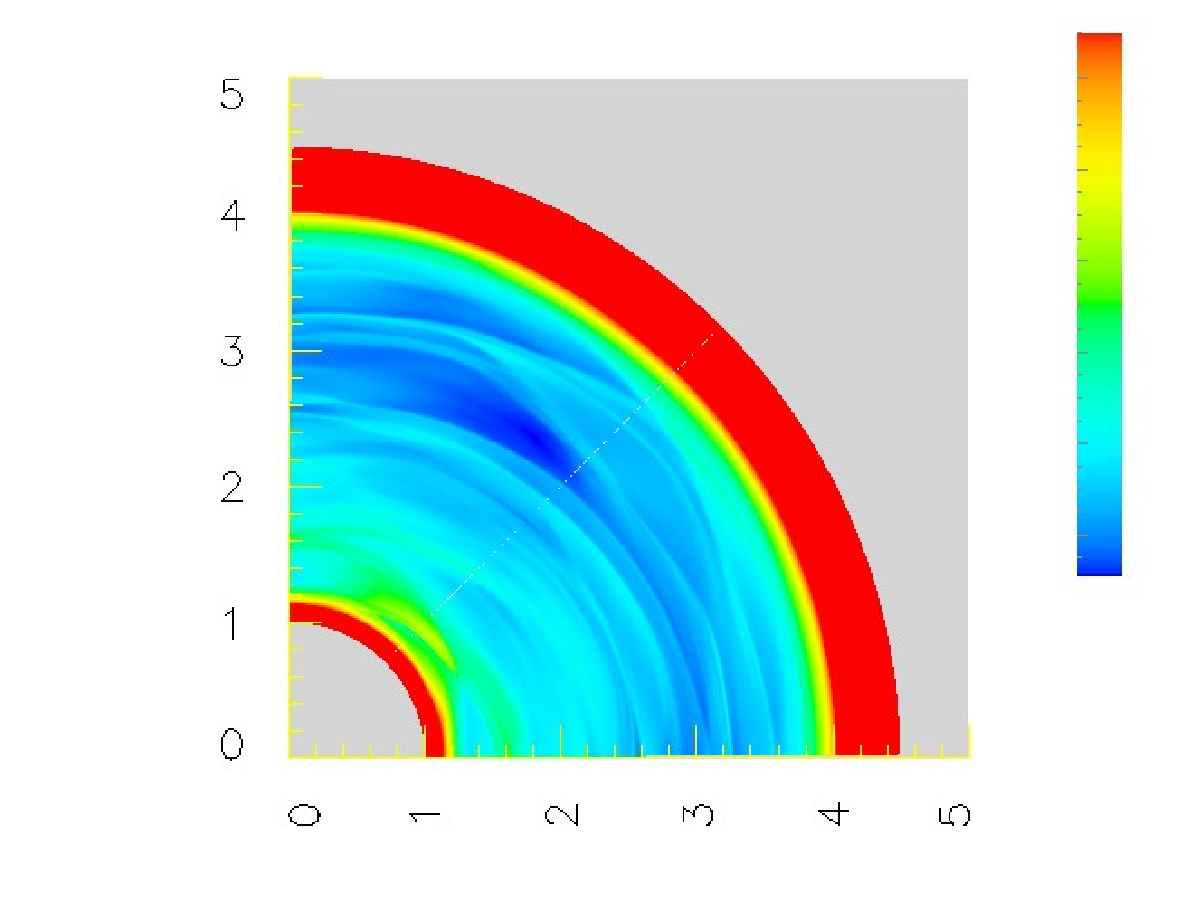
\includegraphics[scale=0.6]{c1fig2.eps}}
\caption{
Vertically averaged density for a cylindrical turbulent 3D-MHD disk using the 
newly developed code {\tt Tramp-MP}. The radial range extends from 1.0 to 4.5
in dimensionless units. At the inner and outer boundary the turbulence is
switched off by using a constant angular velocity profile, which leads to high
densities there.
}
\label{fig:c1_2}
\end{figure}

%
% Here follows the own refereed publications by the PIs in relation to
% the project proposed here.
%
\ownpubltitle{Own publications related to the Forschergruppe:}
%
% BELOW IS ONLY AN EXAMPLE OF TWO ENTRIES. SEE THE ADDITIONAL FILES 
% SENT TO YOU WITH ALL THE REFERENCES FROM THE VORANTRAG
%
\begin{ownpubl}
% CPDADD
\item Bell, K.~R., Cassen, P.~M., Klahr, H.~H. and Henning, Th. (1997) 
The Structure and Appearance of Protostellar Accretion Disks: 
Limits on Disk Flaring. \apj, \textbf{486}, 372
%
\item {D'Angelo}, G., Henning, Th. \& {Kley}, W. (2002)
  Nested-grid calculations of disk-planet interaction,
  \aap, \textbf{385}, 647
%
\item {D'Angelo}, G., Henning, Th. \& {Kley}, W. (2003)
  Thermohydrodynamics of Circumstellar Disks with High-Mass Planets,
  \aap, \textbf{599}, 548
%
\item {D'Angelo}, G., {Kley}, W. \& {Henning}, T. (2003)
  Orbital Migration and Mass Accretion of Protoplanets in
  Three-dimensional Global Computations with Nested Grids,
  \apj, \textbf{586}, 540
%
\item  Dziourkevitch, N.  \& Klahr, H. (2005)
  Global MRI in Stratified Proto-Planetary Disks, 3D Simulations,
  Protostars and Planets V, Proceedings of the 
  Conference held October 24-28, 2005 in Hawaii.
  LPI Contribution No.~1286., p.8507, 8507 
%
\item G\"unther, R. (2004)
  Three-Dimensional Parallel Hydrodynamics and Astrophysical Applications,
  Phd-thesis, Eberhard-Karls-Universit\"at T\"ubingen
%
\item Johansen, A. and Klahr, H. (2005) Dust diffusion in protoplanetary discs by
magnetorotational turbulence. \apj, \textbf{634}, 1353-1371.
%
\item Johansen, A., Klahr, H. and  Henning, Th. (2006) 
Gravoturbulent formation of planetesimals. \apj, \textbf{636}, 1121-1134.
%
\item Johansen, A., Henning, Th. and  Klahr, H. (2006) 
Dust sedimentation and self-sustained Kelvin-Helmholtz turbulence
in protoplanetary disk mid-planes. 
I. Radially symmetric simulations. \apj, in press
%
\item Johansen, A., Klahr, H. and Mee, A.J. (2006) 
Diffusion properties of magnetorotational turbulence in accretion disks:
Effects of an imposed magnetic field. \mn, in press, 
ArXiv Astrophysics e-prints arXiv:astro-ph/0603765
%
%
\item Klahr, H. and Henning, Th. (1997). 
Particle-trapping eddies in protoplanetary accretion disks,
\ica, \textbf{128}, 213--229.   % c04 - Klahr
%
\item Klahr, H. (1998)
Thermische Konvektion und Staubteilchenverteilung in protoplanetaren Akkretionsscheiben
Phd-thesis, Universit\"at Jena
%
\item Klahr, H.,  Henning, Th. \& Kley, W. (1999)
 On the Azimuthal Structure of Thermal Convection in Circumstellar Disks,
 \apj, \textbf{514}, 325
%
%CPDADD
\item Klahr, H. \& Bodenheimer, P. (2003)  Turbulence in accretion disks:
vorticity generation and angular momentum transport via the global
baroclinic instability. \apj, \textbf{582}, 869
%
\item Klahr H. \& Lin, D.~N.~C. (2005) Dust Distribution in Gas Disks II: Self 
Induced Ring Formation through a Clumping Instability. \apj, \textbf{632}, 
1113-1121.
%
%
\item Klahr,H. \& Kley, W. (2006)
 3D-radiation hydro simulations of disk-planet interactions. 
  I. Numerical algorithm and test cases,
  \aap, \textbf{445}, 747
%
\item Klahr, H. \& Bodenheimer, P.\ (2006)\ 
Formation of Giant Planets by Concurrent Accretion of Solids and Gas inside
an Anticyclonic Vortex.\ \apj, \textbf{639}, 432-440.
%
\item Klahr, H., Rozyczka, M., Dziourkevitch, N., W\"unsch, R., Johansen, A.\ 2006.\
Turbulence in Protoplanetary Accretion Disks: 
Driving Mechanisms and Role in Planet Formation.\ in  {\em Planet Formation},
Edited by Hubert Klahr and Wolfgang Brandner, pp.~.~ISBN 0521860156.~Cambridge, UK 
Cambridge University Press,  2006.\ . 
%
\item Kley, W. (1999)
  Mass flow and accretion through gaps in accretion discs,
  \mn, \textbf{303}, 696
\item Kley, W., {D'Angelo}, G., \& {Henning}, T. (2001)
  Three-dimensional Simulations of a Planet Embedded in a
   Protoplanetary Disk,
  \apj, \textbf{547}, 457
\item Kley, W. \& Lin, D.N.C. (1996)
  The Structure of the Boundary Layer in Protostellar Disks,
  \apj, \textbf{461}, 933
\item Kley, W. \& Lin, D.N.C. (1999)
  Evolution of FU Orionis Outbursts in Protostellar Disks,
  \apj, \textbf{518}, 833
\item Kley, W., Papaloizou, J.C.B. \& Lin, D.N.C. (1993)
 On the Angular Momentum Transport Associated with Convective
  Eddies in Accretion Disks,
  \apj, \textbf{416}, 679
\item Nelson, R.~P., {Papaloizou}, J.~C.~B., {Masset}, F.~S. \& Kley, W. (2000)
  The migration and growth of protoplanets in protostellar discs,
  \mn, \textbf{318}, 18
%
\item W\"unsch, R., Klahr, H.~H., and R\'o\.zyczka, M. (2005) 2-D models of layered
protoplanetary disks: I. The ring instability. \mn,  \textbf{362}, 361-368.
%
\item  W{\"u}nsch, R., Gawryszczak, A., Klahr, H., R{\'o}{\.z}yczka, M.\ (2006) 
Two-dimensional models of layered protoplanetary discs - II. The effect of a residual 
viscosity in the dead zone.\ \mn, \textbf{367}, 773-780.\
%
\end{ownpubl}
%
\section{Goals (Ziele)}
%
Within this project we plan to investigate, using {\it local and global}
numerical magnetohydro\-dynamical simulations, how the spatial distribution
and velocity distribution of dusty agglomerates within a protoplanetary disk
is affected by the turbulent motions of the gas.  The results shall be used,
in combination with the results from the experimental projects (B1, B2), to
create a coagulation kernel for the project C2.  Both, the fluctuating
collisional velocities and the fluctuating particle densities have to be
translated into an effective collision rate and sticking probability.  The
detailed fashion, how this translation can be achieved must be developed,
after we have performed the relevant direct numerical simulations.

We plan to perform complementary analysis by utilizing two different
approaches.  In Heidelberg at the Max-Planck Institut f\"ur Astronomie
(MPIA) {\it local} accretion disk simulations with embedded dust will be
performed, while at the Institute for Astronomy \& Astrophysics in
T\"ubingen (IAAT) fully {\it global} disk models will be constructed.  In
the first case we will have a higher resolution and better coverage of
statistics, while in the latter case we can focus on the global disk
effects.  This two-fold approach will enable us to obtain reliable estimates
on the statistical properties and efficiency of the MHD-turbulence in
protoplanetary accretion disks on the global as well as on the local scale,
and allow firm conclusions on the distribution of dust and boulders within
such disks.
% 
%
\begin{itemize}
\item Objective 1: {\sf Collision velocities and rates}\\
{\em Local} simulations of MHD unstable (turbulent) disks are to be
performed in Heidelberg at the MPIA, where we will treat the dust as
individual particles and follow its distribution by direct numerical
integration of the relevant equations including the interaction forces
between the gas and the dust.  As a result of the computations we will
determine the collision rates and relative velocities which play the
dominant role in the subsequent growth phase.
%
For this part of the project we will use our standard set up of local MHD
simulations. The new part will be the implementation of special measurement
tools for the individual encounter rates and velocities of the
particles. Huge amounts of data will be produced in these simulations, that
has to be interpreted with the proper statistical tools. One issue that has
to be investigated is the influence of our limited spectral range of the
turbulence on the relative velocities between the particles.  In particular,
for small particles that couple mostly to smaller length-scales than those
which are resolved one has to modify our approach of direct simulation of
turbulence. Here we plan to ``zoom'' into smaller scales of the turbulence
and neglect the larger (here unimportant) scales, but incorporate their
effect as an external forcing acting on our small box.  Settling and radial
drift can also be added, thus we will compile all the relevant local
parameters for collisions of planetesimal precursors in protoplanetary
disks.
%
\item Objective 2: {\sf Global distribution, size segregation and local
enhancement}\\ 
%
In this part of the joint project we plan to perform {\em Global} simulations
of magnetized, turbulent protoplanetary disks at the IAAT.  These
simulations will include the radial gradients (eg. differential rotation,
density and temperature profiles) in accretion disks and also a realistic
vertical stratification of the disk.  In contrast to project A2 where the
turbulence is parameterized as an effective ($\beta$-type) viscosity, we
will perform here direct numerical simulations of 3D magneto-hydrodynamical
disks. This may imply that the simulations in A2 are able to cover a larger
radial range of the disk and longer time scales, but without any azimuthal
information.
%% The two approaches can be viewed as complementary approaches.

Our new models aim towards a self-consistent treatment of turbulent disks
where the turbulent energy which is dissipated on small scales is fed back
as heat into the system, and is finally released through radiation. There
are no simulations so far in the literature that combine radiation transport
and magneto-hydrodynamics for protoplanetary disk studies.  The main
problem will consist in the combination of numerical algorithms that are
available in our two groups, and that will have to be put into a modern
computational framework and have to be parallelized.  The evolution of
embedded dust in such a fully turbulent global disk will then be followed.

\noindent
The following challenges have to be met:
%
\begin{itemize}
\item Add a module for following the evolution of embedded dust 
\item Analyze the dust distribution within the turbulence
\item Develop a parallel module for solving the radiative transport in the
 flux-limited diffusion approximation
\item Add opacities and realistic equation of state 
\item Include non-ideal effects (dissipation of kinetic and magnetic energy)
  and construct self-consistent accretion disk models
\end{itemize}

\end{itemize}
%
\section{Work schedule (Arbeitsprogramm)}
\subsection{Methods}
\subsubsection{Local Disk Simulations}
Johansen \& Klahr (2005) have performed {\em local} 3D-MHD simulations of
turbulence in accretion disks and measured the diffusion of dust induced by
the turbulence. They also studied the local concentration of meter-sized
objects in 3D-MHD turbulence by simulating $2\times 10^6$ particles
(Johansen, Klahr \& Henning 2006).  These simulations will be the starting
point for Objective 1 of this new project. The problem is very challenging
because
\begin{itemize} 
\item{particle sizes are many orders of magnitude smaller than the typical box size of such
simulations,}
\item{despite the huge number of $2\times 10^6$ particles, one is still many orders below realistic particle numbers,}
\item{and additionally the smallest scales of the turbulence can usually
not be resolved.} 
\end{itemize}
%
To overcome these obstacles we will apply two techniques: First, we will use
the concept of ``super-particles'' where one particle actually mimics an
entire flock of e.g.\ meter sized boulders, which move on a similar
path. The super-particle concept has been used successfully in plasma-physics
for many years (Birdsall \& Langdon 1985).

And second, we will perform separate simulations for the many scales of
turbulence.  Particles couple always strongest to a preferred eddy
frequency i.e.\ a certain length scale of the turbulence, where the friction
time of the particles equals the correlation time of the turbulence on that
specific scale.  This effect will give a lever to disentangle different
parts of the turbulence cascade for the relevant particle sizes.  The
strategy is to resolve not all the scales at once, but only the scales which
are important for the chosen particle size.  The effect from larger and
smaller scales can then be included via external forcing (larger scales) and
via sub-grid modeling (smaller scales).

As a final step, effects of particle growth will be included in a simplified
way, i.e.\ the individual size of the objects within a super-particle can
increase if a collision was soft enough, or decrease if the collision was
destructive.

We usually simulate the protoplanetary disk in the shearing sheet
approximation (Goldreich \& Tremaine 1978; Brandenburg et al.\ 1995; Hawley
et al.\ 1995). Here a local coordinate frame corotating with the disk with
the Keplerian rotation frequency $\varOmega_0$ at a distance $r_0$ from the
central source of gravity is considered. The coordinate system is oriented
so that $x$ points radially away from the central source of gravity, $y$
points along the Keplerian flow and $z$ points perpendicular to the disk
along the Keplerian rotation vector {\boldmath $\varOmega_0$}. As a
numerical solver we use the Pencil Code, a finite difference code that uses
sixth order symmetric space, derivatives and a third order time-stepping
scheme (see Brandenburg 2003).

The dust component is represented by typically 2,000,000 numerical particles
each with an independent position ${\bf{x}}^{(i)}$ and velocity vector ${\bf
v}^{(i)}$. The gas acts on the dust particles through a drag force that is
proportional to, but in opposite direction of, the velocity difference
between a dust grain and the surrounding gas. The equation of motion of the
dust particles is
\begin{equation}
 \frac{d {\bf v}^{(i)}}{d t} = {\bf f}({\bf v}^{(i)})
      - \frac{1}{\tau_{\rm f}} \left({\bf v}^{(i)}-{\bf u}\right) + {\bf g}\, ,
  \label{eq:eqmotp}\\
\end{equation}
where $\tau_{\rm f}$ is the {\it friction time} and $\bf{g}$ is an imposed
gravity field (see below). The term ${\bf f}({\bf v}^{(i)})$ stands for the
Coriolis forces and the shear potential necessary for the shearing sheet box
simulations (see Johansen et al.\ 2006 for a detailed definition).  In most
cases we can assume that $\tau_{\rm f}$ is a constant that is independent of
the relative velocity between the grain and the surrounding gas. In
protoplanetary disks this is a valid assumption for sufficiently small and
slow dust grains (Weidenschilling 1977). This is the case both in the
Epstein regime, where the particle is smaller than the mean free path of the
gas molecules and in the Stokes regime, where the particle is larger.  In
the Epstein regime individual collisions of the gas molecules with the grain
surface transfer the momentum, where as in the Stokes regime a laminar flow
develops around the body, producing a pressure gradient around the body. We
usually use a value of $\varOmega_0 \tau_{\rm f} < 10.0$.  Larger particles
with a more complicated aerodynamical coupling to the gas can be considered,
too. The relevant friction laws can be found in detail in Weidenschilling
(1977).

The particles change positions according to the dynamical equation
\begin{equation}
  \frac{d {\bf x}^{(i)}}{d t} = {\bf v}^{(i)} + u_y^{(0)} \hat{\bf{y}} \, .
\end{equation}
Based on these simulations we will be able to measure the desired quantities
to characterize collisions between planetesimal precursors.  Therefore, we
have to implement the measurement tools in an efficient way. The statistical
analysis tools have to be developed and simulations for various particle
sizes have to be performed, first for mono dispersive particle
distributions, and later for particle size distributions.  It will be
interesting to compare our measurements to the analytical estimations by
Markiewicz et al.~(1991), Mizuno et al.~(1988) and V\"olk et al. (1980).

We also will have to study the influence that spatial resolution has on
our results, especially as a complete coverage of the turbulent spectrum
is impossible for one single simulation. 

The master simulation is based on the models from year one. Now new models
are generated, which use only 0.1 pressure scale heights for the box size of
the computational domain instead of 1 pressure scale height in the master
model, but the identical number of grid cells.  Thus, the individual time
step is 10 times smaller, but on the other hand the relevant time scale,
e.g.\ sound crossing times and shear times are also down by a factor of
ten. The resulting total computational effort is not higher than in the
master model.  Now the resolution is 10 times better and one follows one
order of magnitude further down the turbulent cascade. The influence of the
larger scales is given by external forcing at a strength that is determined
by the master simulation. With this second simulation one can already study
what the effect of turbulence on these smaller scales has on particle
collisions in dependence of their size.

This process can be iterated for the next smaller scales by using the second
simulation as the new master simulation for the third simulation. In roughly
10 steps it will then be possible to resolve the entire cascade down to the
dissipation scale. This process has to be controlled for consistency by
e.g.\ checking the combined spectral energy distribution of the turbulence
from all the simulations. This can be compared to analytical predictions,
e.g.\ the Kolmogorov law and at least in part comparing it to spectra
obtained for high resolution simulations of turbulence. Simulations without
particles can be performed at much higher resolution, because the
computational effort is less in such a case and the simulation can also be
about 10 times shorter than in case one studies the statistical properties
of the dust.

For large particles only the largest velocities will be important, which
happen to be the largest scales, thus already resolved in the largest
box. But smaller and smaller particles couple to smaller and smaller scales
in a sense that they receive their turbulent relative (collision) velocity
only from scales, which are normally neglected in such simulations, but will
be fully covered in our project.

%
\subsubsection{Global Disk Simulations}
%
As pointed out above, even for very simple equations of state (isothermal
configurations) there are only very few existing accretion disk simulations,
most of them with no or only approximate vertical gravity.  Here, we will
focus on constructing {\it realistic models} of radially and vertically
stratified disks.

These planned {\em global} simulations of Objective 2 will be very demanding
computationally as larger physical scales and longer time-scales will have
to be covered by the calculations.  This is feasible only by utilizing very
efficient, highly parallelized codes.  Based on the existing code TRAMP
(Klahr et al.\ 1999), we have already developed a completely parallel
version {\tt Tramp-MP} which solves the 3D hydrodynamical equations
including self-gravity in arbitrary coordinates (G\"unther 2004).  The code
is based on a modern, modular algorithm written in the C++ language which
allows efficient programming using template structures and operator
overloading.  Parallelization is achieved using the library POOMA (Atlas et
al.\ 1995), which is ideally suited to develop parallel algorithms for
grid-based codes using distributed memory.  This new parallel code has been
successfully extended by us to a full 3D-MHD code that has been used to
study the Magneto Rotational Instability in isothermal global disks (Marik
et al.\ 2006, in prep.).

Within this project, efforts and expertise in Heidelberg and T\"ubingen will
be combined and the {\tt Tramp-MP}-code will extended by a by including {\it
radiative transport} in the flux-limited diffusion (FLD) approximation
similar to Klahr et al.\ (1999).  For the main part of the accretion disk
which is optically thick this approach is well justified.  At the same time
we shall implement a more realistic {\it equation of state} and {\it
opacities}, necessary for the proper radiation treatment.  To avoid too
stringent time-step limitation the radiation part will have to be solved
implicitly, which is a non-trivial task in a parallel environment. We will
base our linear equations solver on existing libraries that we utilize
already for the Poisson-solver (G\"unther 2004).  In test calculations the
newly developed module will be applied to a standard disk setup and compared
to results obtained with the 2D-code of project A2.

To obtain a self-sustained turbulent state the kinetic energy contained in
the turbulent motion has to be converted into thermal energy at the small
spatial scales. This can be achieved by including for example {\it
non-ideal} MHD-effects such as magnetic diffusion and viscosity, which
converts magnetic and kinetic energy into heat. In its present version the
code can work with either the thermal energy equation of the total
mechanical energy (thermal plus kinetic). If required to ensure better
energy conservation, the option of using a total energy equation (adding
magnetic energy) has to be considered.

In close collaboration with the first part of the project (Objective 1) we
will focus on the motion of dust in a turbulent disk.  The interaction of
the embedded dust with the flow can be incorporated in these global models
by a continuum approach by using an additional scalar field for the dust or
by explicit integration of up to currently $2 \times 10^6$ individual
particles. The important transport coefficients for the continuum approach
will be obtained from local simulations which are part of Objective 1 of
this project (see also Johansen \& Klahr 2005).

\subsection{Schedule Student 1 (located at the MPIA)}
\subsubsection{First year} 
The first goal for the student is to learn how to work with the Pencil Code
(1st three months).  The code is well documented and we have experienced
users and even developers at the MPIA. On top of that, there is an active
user group that is regularly discussing problems with the code and provides
support to each other.  The student will also have to gather experience in
the usage of the 256+8 processor computing cluster PIA and in the handling
and interpretation of the produced data.

As the initial step towards own research the student can measure relative
velocities in the existing models of turbulent disks. One has to understand
how to measure these root-mean-square velocities and how they fluctuate over
time and space (2nd three months).  In the next step these fluctuations have
to be measured and interpreted in a Lagrangian sense, i.e.\ one has to
follow the individual particles and measure the r.m.s.\ velocities and
particle densities that they experience in dependence of time.  This means
that the student has to implement suitable algorithms to efficiently measure
fluctuating collision rates, the fluctuating relative velocities and the
correlations among these values for various particle sizes.

Together with our partners in project B1, B2, B4 and especially C2 we will
discuss how to formulate a coagulation kernel from these data, especially
how our measurements compare to the analytical estimations by Markiewicz et
al.~(1991).  The experimental and numerical projects on collisions (B1, B2,
B4) will deliver critical velocities for sticking, bouncing and destruction
that have to be folded with our correlations of densities and velocities in
order to generate a coagulation kernel for C2 that only depends on the mean
particle densities and a general turbulence parameter.
 
We will then also learn what the influence of numerical parameters like
resolution and size of the computational domain are, as well as how the
effects from physical parameters like a global field strength influence our
results.  Performing the simulations for wide parameter ranges and providing
these data sets to the other groups within the Forschergruppe is the final
goal for the first year.
\subsubsection{Second year} 
Now we have to expand our local simulations of MHD turbulence in
protoplanetary disks with vertical stratification and possibly also
non-ideal MHD effects to treat an inactive mid-plane layer (four
months). The physics of e.g.\ resistivity have to be tested and verified.

The student will also develop new MHD box models that follow the turbulent
cascade down to the dissipation scale by using input (driven turbulence)
from simulations at larger scales (about four months). 


\subsubsection{Third year}
As a final goal one can now combine the MHD simulations with simulations for
the dust growth.  In that case we use the results from B1, B2 and C2 to
allow our particles to bounce, stick or destroy each other in the course of
their collisions. The small debris can feed the dust background continuum,
treated as a mass density, which is also advected.  It will also be possible
that the large bodies sweep up the small debris, thus growing in size while
depleting the back ground.  In that fashion it should be possible to let the
particles represented in the super particles grow from about 0.1 meters up
to 10 meters, which is actually the most critical part of the growth as
usually the collision velocities are too high for growth (see introduction)
as well as the radial drift rates have a maximum, which leads to a huge
particle loss towards the central object.

%%In the aftermath the student will have time
%%to write up the thesis in the last six months.

\subsection{Schedule Student 2 (located at the the University of T\"ubingen)}
\subsubsection{First year} 
In the initial phase the student has to familiarize him/herself with the
operation of the existing code {\tt Tramp-MP}. The code is well documented
and kept up to date using a CVS repository used jointly by the involved
scientists in Heidelberg and T\"ubingen.  In this first phase, the student
is expected to simulate models of global vertically stratified accretion
disks in the present code-setup using spherical polar coordinates. Here the
student will gain experience with in-output and post-processing, and
understand the internal structure and functioning of the code. By
implementing new boundary conditions on the magnetic field configurations
already new and interesting astrophysical results will be obtained.  We
estimate that this part may take about a quarter to half a year.

It will be followed by incorporation of radiative transport (flux-limited
diffusion) into the existing parallel code {\tt Tramp-MP}.  The
implementation has to be implicit which leads for a finite difference scheme
to a large system of linear equations, to be solved at each time step.  We
plan to use existing routines for example from the {\tt TIPSY} library which
have been developed particularly for MPI implementations.  The internal link
to such routines has been prepared already within the Poisson-solver routine
(G\"unther 2004). It needs to be adapted for the solution of the equations
resulting from the diffusion approximation.  The newly implemented part of
the code needs to be tested and results compared to other existing models of
(hydrodynamic) radiative disks.  This part of the project is based on our
great experience in flux-limited diffusion in 2D and 3D simulations, and
both partners in Heidelberg and T\"ubingen will actively work on this
project.  Hence, we estimate that, despite its complexities, it may take
including testing only about half a year to nine months.
%
\subsubsection{Second year} 
%
Parameter studies of fully radiative disks will be performed for different
field configurations (eg. zero net flux condition, or vertical fields).  The
statistical properties of the turbulence (total magnetic, kinetic energies,
angular momentum transport, ...) will be analyzed. We expect to arrive at
new quantitative predictions for equilibrium structures of protoplanetary
disks with respect to the magnitude of the effective $\alpha$ and its
thermal structure.

In parallel to these parameter studies we will begin with implementing a
solver to evolve the dust in such a disk. This part is based on our
experience obtained in the local simulations (at the MPIA) in which such
solvers have already been developed and used in several simulations.  We
plan to first use the continuum approach and use available results on
diffusion properties and algorithmics from the first part of the project.
For larger particle sizes the implemented particle solver from Objective 1
can be utilized.
%
\subsubsection{Third year} 
We shall perform parameter studies of global protoplanetary disks with
embedded dust.  We will analyze the statistical distribution and velocity
dispersion of the dust, and will compare results in detail with the local
runs in Objective 1.  We will examine the possibility of particle trapping
in long-lived turbulent eddies or vortices.  The possibility of rapid planet
formation through dust enhancement will be analyzed.  In case time will be
left in the project we will analyze the influence an existing planet has on
the dust distribution. In particular if this may lead to induced secondary
planet formation, and we would like to study the observational impact of an
embedded planet in a dusty disk.
%
\subsection{Literature}
%
% Here follows a general literature list related to the topic of the
% BIS HIER KAM ICH!!! HUBERT !!!
% proposal, just like a literature list for a scientific paper.
%
% AGAIN ONLY EXAMPLES ARE LISTED NOW
%
\begin{literature}
\item Arlt, R., \& R{\"u}diger, G.\ (2001) Global accretion disk simulations of 
magneto-rotational instability.\ \aap, \textbf{374}, 1035-1048. 
 
\item Armitage, P.J. (1998)
  Turbulence and Angular Momentum Transport in Global Accretion Disk Simulation
  \apj, \textbf{501}, L189
\item Atlas, S. et al., (1995)
   POOMA: A high performance distributed simulation environment for
   scientific applications, in {\it Proceedings of SuperComputing 95},
   see {\tt http://www.nongnu.org/freepooma/}
\item Balbus, S.~A., \& Hawley, J.~F. (1991) 
   A powerful local shear instability in weakly magnetized disks. I - Linear analysis,
  \apj, \textbf{376}, 214
\item Birdsall,C.K., \& Langdon, A.B., (1985) Plasma physics via computer simulation,
McGraw Hill, 1985
\item Brandenburg, A., Nordlund, A., Stein, R.~F., Torkelsson, U.\ (1995) Dynamo-generated 
Turbulence and Large-Scale Magnetic Fields in a Keplerian Shear Flow,
  \apj, \textbf{446}, 741. 
\item Brandenburg, A.\ (2003)
Computational aspects of astrophysical MHD and turbulence.\ Advances in 
Nonlinear Dynamics , \textbf{269}. 
\item Carballido A., Stone J.~M., \& Pringle J.~E. (2005) 
  Diffusion coefficient of a passive contaminant in a local MHD model of a turbulent accretion disc,
  \mn, {\bf 358}, 1055
\item  Dominik, C., Blum, J.,  Cuzzi, J., , \& Wurm, G.\ (2006) 
  Growth of Dust as the Initial Step Toward Planet Formation,
  ArXiv Astrophysics e-prints arXiv:astro-ph/0602617. 
\item Dullemond, C.~P., Apai, D., Walch, S.\ (2006) 
   Crystalline Silicates as a Probe of Disk Formation History,
   \apj {\bf 640}, L67
\item Fromang, S. \& Nelson, R.~P.\ 2005.\ On the accumulation of solid bodies in global 
turbulent protoplanetary disc models.\ \mn \textbf{364}, L81-L85. 
% 
\item Fromang, S., \& Papaloizou, J.\ (2006) Dust settling in local simulations of turbulent 
protoplanetary disks.\ ArXiv Astrophysics e-prints arXiv:astro-ph/0603153. 
%
\item Goldreich, P., \& Tremaine, S.\ 1978.\ The excitation and evolution of density waves.\ \apj, \textbf{222}, 850-858.  
%
\item Hawley, J.~F., Gammie, \& C.~F., Balbus, S.~A.\ (1995) Local Three-dimensional Magnetohydrodynamic 
Simulations of Accretion Disks, \apj, \textbf {440}, 742. 
% 
\item Hawley, J.F. (2000)
  Global Magnetohydrodynamical Simulations of Accretion Tori
  \apj, \textbf{528}, 462
\item Ilgner, M., Henning, T., Markwick, A.~J., Millar, T.~J. (2004)
   Transport processes and chemical evolution in steady accretion disk flows,
  \aap, \textbf{415}, 643
\item Ilgner, M., Nelson, R.~P.\ (2006a) On the ionisation fraction in protoplanetary disks. I. 
Comparing different reaction networks,
  \aap, \textbf{445}, 205
\item Ilgner, M., Nelson, R.~P.\ (2006b) 
  On the ionisation fraction in protoplanetary disks. II. The 
  effect of turbulent mixing on gas-phase chemistry,
  \aap, \textbf{445}, 223
\item  Johansen, A., Andersen, A.C. and Brandenburg, A. (2004). 
 Simulations of dust-trapping vortices in protoplanetary discs, 
\aap, \textbf{417}, 361--374.   % c04 - Klahr
%
\item Markiewicz, W.~J., Mizuno, H., \&Voelk, H.~J.\ (1991) Turbulence induced relative velocity 
between two grains.\ \aap \textbf{242}, 286-289. 
% 
\item Mizuno, H., Markiewicz, W.J., \& V\"olk, H.J. (1988), 
 Grain Growth in Turbulent Protoplanetary Accretion Disks, 
  \aap,  {\bf 195}, 183  % c07 - Henning
\item Nelson, R.P. \& Papaloizou, J.C.B. (2003) 
  The interaction of a giant planet with a disc with MHD turbulence -
   II. The interaction of the planet with the disc
  \mn, \textbf{339}, 993
\item Papaloizou, J.C.B. \& Nelson, R.P. (2003) 
  The interaction of a giant planet with a disc with MHD turbulence -
   I. The initial turbulent disc models
  \mn, \textbf{339}, 983
\item Rodmann, J., Henning, T., Chandler, C.~J., Mundy, L.~G., Wilner, D.~J.\ (2006) 
  Large dust particles in disks around T Tauri stars,
  \aap {\bf 446}, 211
\item Steinacker, A. \& Henning, T. (2001)
  Global Three-dimensional Magnetohydrodynamic Simulations of Accretion Disks
 and the Surrounding Magnetosphere
  \apj, \textbf{554}, 514
\item Stone, J.M. \& Norman, M.~L (1992)
  ZEUS-2D: A Radiation Magnetohydrodynamics Code for Astrophysical Flows
  in Two Space Dimensions. II. The Magnetohydrodynamic Algorithms and Tests
  \apjs, \textbf{80}, 791
%
\item Tennekes, H., \& Lumley, J.~L. (1972) First Course in Turbulence
      (Cambridge: MIT Press, 1972)
\item Turner, N.~J., Willacy, K., Bryden, G., Yorke, H.~W. (2006)
   Turbulent Mixing in the Outer Solar Nebula,
  \apj,  {\bf 639}, 1218
\item V\"olk, H.J., Jones, F.C., Morfill, G.E., \& R\"oser, S. (1980),
  Collisions between Grains in a Turbulent Gas, 
  \aap, {\bf 85}, 316   % c07 - Henning
%
\item Weidenschilling, S.~J.\ (1977) Aerodynamics of solid bodies in the solar nebula,
  \mn, {\bf 180}, 57-70. 
%
\end{literature}
%
\section{External/International collaborations}
\begin{collablist}
\item[London] We will work with Richard Nelson (QMUL) on turbulent MHD disks and particle-gas interaction.
\item[Paris] We work together with Steve Balbus on non ideal effects in accretion disks.
\item[Pasadena] We have ongoing collaborations with Neal Turner and Geoff Bryden
on Radiation Magnetohydro Simulations of Accretion disks, where we share code and experience.
\item[Potsdam] We will work with the group of Udo Ziegler on numerical MHD.
\item[Prague] Richard Wunsch is also part of the TRAMP developer and user team for
  global simulations of global accretion disks.
\item[Santa Cruz] Here we study with Doug Lin the dust distribution in optical thin but gaseous disks
with analytic and numerical methods. We also study the influence
of local dust enhancement on the core accretion model for planet formation together with Peter Bodenheimer.
\end{collablist}
%
%
\section{Link to other projects of the Forschergruppe}
\begin{linkproj}
\item[\projtscharn{}] Exchange ideas and numerical expertise concerning the
the energy transport via radiation. Define a joint test problem involving a
standard disk setup.
\item[\blockimpact{}] The derived collision velocities and rates will be
used as input and parameter guideline for the setup in
collision experiments (B1-B3, Wurm, Blum, Trieloff), and also for
the initial conditions in the numerical simulations (B4, Kley \& Speith).
On return we will use their results on the probabilities for sticking,
bouncing and destructive collisions in dependence of velocity to
fold these values with our measured velocities. 
%
\item[\projdul{}] The collision rates and velocities will be vital input for
the description of the particle growth via a coagulation equation approach.
The statistical description of the inhomogeneities, e.g.\ an intelligent
integral of the fluctuating values will be used to generate a coagulation kernel.
This kernel can then be
used in project \projdul{} to model coagulation globally in space and time.
%
\item[\projtrie{}] Predictions of the speed with which planetesimals form
(dominated by the bottle neck at 1 meter in size)
can be compared to the formation times scales of planetary cores
as obtained from radiometric dating (project \projtrie{}).
%
\item[\projwolf{}] Predictions of inhomogeneities of the dust
distribution due to particle trapping, in particular cm-sized pebbles in the
outer regions of disks, will be used in project \projwolf{} to test the
observability of such particle trapping mechanisms.
%Predictions of where in the disk, and how often, meter
%sized bodies collide and produce observable dust will be used by project
%\projwolf{}.
\end{linkproj}
%
\section{Team members (Zusammensetzung der Arbeitsgruppe)}
%
% NOTE: Only list non-DFG-funded team members.
% NOTE: Also list technical assistants, students etc involved in the project
%
\begin{teamlist}
% -> Willy, some notes?
\item[Klahr, H.~H., Dr.]\mbox{}\\
Team leader. Supervises the first PhD student at the MPIA which is
not funded through the project.
Provides excellent knowledge about the dust dynamics in turbulent
protoplanetary accretion disks.
\item[Kley, W., Prof.~Dr.~(C4)]\mbox{}\\
Team leader. Supervises the PhD student in T\"ubingen
funded through the project. Provides extensive expertise in
theory of accretion disks, planet formation, computational astrophysics
and numerical aspects.
\item[Johansen, A., PhD student]\mbox{}\\
Internal collaborator. Provides extensive knowledge about local
3D MHD calculations using the {\tt Pencil} code, including the
motion of embedded dust particles.
\item[Dziourkevitch, N., Postdoc]\mbox{}\\
Internal collaborator. Provides extensive knowledge about
3D MHD calculations using the {\tt ZEUS-MP} code, including 
non-ideal MHD effects.
\item[Marik, D., Postdoc]\mbox{}\\
Internal collaborator. Provides extensive knowledge about
3D MHD calculations using the {\tt Tramp-MP} code.
\item[Hofrichter, C., Student]\mbox{}\\
Internal collaborator. Provides extensive knowledge about
programming issues using C++ and the {\tt Tramp-MP} code..
\item[Speith, R., Dr.]\mbox{}\\
Internal collaborator. Provides extensive expertise in numerical particle methods.
Has widespread experience in parallel computing for
shared memory architectures using OpenMP directives and distributed
memory architectures with the Message Passing Interface (MPI).
\end{teamlist}
\vspace{1em}
%
\section{Funding requested}
We request funding for only {\em one} of the two PhD student positions for
this project (in T\"ubingen). The second one (Heidelberg) will be financed by the host
institution (MPIA).  The following table gives the full overview of requested
funding:\vspace{1\baselineskip}\\
%
% The table that follows is the overview over the full requested 
% funding, including the positions, travel, consumables and ``other
% costs'' (which might include transportation costs of radioactive
% material or the rent of a drop tower or such).
%
\centerline{\begin{tabular}{||l|r|r|r||} \hline \hline & Year 1 & Year 2 &
Year 3 \\ \hline %
Personnel (1 PhD-students: E13/2)   & \hfil 24.000 & 24.000 & 24.000 \\
Consumables                        & \hfil 0 & \hfil 0 & \hfil 0 \\
Travel                             & \hfil 2820 & \hfil 2820 & \hfil 2820 \\
Other costs                        & \hfil 4000 & \hfil 0 & \hfil 0 \\
\hline
{\bf Total:} (EUR)                 & \hfil 26.820 & \hfil 26.820 & \hfil 26.820 \\
\hline
\hline
\end{tabular}
}
\vspace{1em}\\
Below these costs are explained in more detail:

\subsection{Personnel (Personalbedarf)}
\begin{teamlist}
\item[PhD-Student 1 (E13/2)]\mbox{}\\
The PhD student in T\"ubingen will extend the existing code {\tt Tramp-MP}
to include radiative transport and an evolution scheme for embedded dust
particles.  He/she will then perform detailed parameter studies of global
radiative disks to determine the distribution of dust in turbulent magnetized
disks disks.
\end{teamlist}
%
\subsection{Consumables (Verbrauchsmaterial)}
none
%
\subsection{Travel expenses in addition to Project Z (Reisekosten)}
%
% Here only travel expenses not related to usual regular Forschergruppe
% meetings and the overall per capita budget for conferences.
%
The project is constructed as a close collaboration between Heidelberg and
T\"ubingen, and we envision frequent visits of the students to the partner
institutes. We plan for two visits for each year and student for one week
each.  And also one trip per year for the team leaders (2 days).  For the
return trip between Heidelberg and T\"ubingen we assume 70 EUR, and a per
diem rate of 100 EUR.  Estimated costs (in EUR) per
year:\vspace{1\baselineskip}\\
\centerline{\begin{tabular}{||l|r|r|r||} \hline \hline & Year 1 & Year 2 &
Year 3 \\ \hline %
%%  \centerline{\begin{tabular}{|p{18em}|p{7em}|p{7em}|}
\hline
4 Travel between partner Institutes (students)  &  \hfil  2280    & \hfil 2280  & \hfil 2280 \\
2 Travel between partner Institutes (leaders)  &  \hfil  540    & \hfil 540  & \hfil 540 \\
\hline
\end{tabular}}
\\[0.3cm]   
%For a trip to Potsdam we assume 150 EUR travel and 100 per diem.  For the
%trips to London and Paris we assume 200 EUR travel costs and 140 EUR per
%diem.  For trips to California we assume 1000 EUR travel and 140 EUR per
%diem.
%
\subsection{Other costs (Sonstige Kosten)}
%
The PhD students in T\"ubingen in Heidelberg require mobile personal
computers (laptops) to work and to present their results during the frequent
visits in Heidelberg and at the other partner institutes.  The cost for
these laptops (MacBook Pro) will be approximately EUR 2000 each.
%
\section{Preconditions for carrying out the project at home institution}
%
% This is one of the main subsections of a DFG Normalverfaren proposal.
% Several of the subsubsections in this subsection we have placed in their
% own subsections above (like team members, collaborations). What remains
% are the following three subsections. For those not familiar with these,
% we refer to the DFG Merkblatt on Normalverfahren-proposals.
%
\subsection{Scientific equipment available (Apparative Ausstattung)}
%
% Please list those larger instrument available to you for the project (if
% applicable also larger computer equipment in case you need substantial
% amounts of computer time).
%
In additions to numerous individual workstations at the Institut f\"ur
Astronomie und Astrophysik T\"ubingen (IAAT) and at the Max-Planck Institut
f\"ur Astronomie (MPIA), we have the following computational equipment
available
%% in T\"ubingen and Heidelberg
\begin{itemize}
\item Beowulf Cluster {\tt phoenix}, 16 dual AMD, IAAT
\item Beowulf Cluster {\tt phoenix II}, 16 Dual Core AMD Opteron 270
with Gigabit interconnections, IAAT
\item Beowulf Cluster {\tt kepler}, 98 dual Pentium-III, 16 dual AMD
with Myrinet interconnections, SFB 382
\item Quad Itanium2 {\tt natasa}, 16 GB Memory, IAAT
\item Cluster {\tt PIA}, 128 Opteron dualboards, plus 2 Opteron quadboards, MPIA
\end{itemize}

Additionally, if required we will apply for computing time at the HLR
Stuttgart in particular for the high resolution simulations.
%
\subsection{Institution's general contribution (Laufende Mittel f\"ur Sachausgaben)}
%
% Please state the annual fund for consumables which comes from the
% institution's budget or any other third party  (please list separately) to
% pay for the research for which your project is part of.  Use estimates where
% applicable. 
%
Student 1 working in Heidelberg will be funded entirely by the host
institution (MPIA).

\medskip

\noindent
The following table gives the additional general contribution from the
institutions budget:\vspace{1\baselineskip}\\
\centerline{\begin{tabular}{||l|r|r|r||}
\hline \hline & Year 1 & Year 2 & Year 3 \\ \hline %
Consumables (MPIA)                 & 500  & 500  & 500  \\
Consumables (IAAT)                 & 500  & 500  & 500  \\
\hline
{\bf Total:} (EUR)                 & 1000  & 1000  & 1000  \\
\hline \hline
\end{tabular}
}

